%==============================================================================
% Document:    
% File:        
% Authors:     
%==============================================================================


%==============================================================================
% Document setup
%==============================================================================

\documentclass[12pt,a4paper]{report}


% Use packages
\usepackage{stys/kiss}
\usepackage{verbatim}
\usepackage{rotating}
\usepackage{color}
\usepackage{a4}
\usepackage{url}
\usepackage{stys/enumerate}
\usepackage{graphicx}
\usepackage{stys/moreverb}
\usepackage{xcolor}
\usepackage[anchorcolor=black,bookmarksnumbered=true,bookmarksopen=true,linkcolor=black,menucolor=black,pagecolor=black,linkbordercolor={1
1 1}]{hyperref}
\usepackage{stys/placeins}
\usepackage{stys/longtable}
\usepackage{caption2}
\usepackage{stys/lipsum}
\usepackage{changepage}
\usepackage{tabulary}
\usepackage{booktabs}

% Specify document wide settings/parameters
\setcounter{secnumdepth}{5}
\setcounter{tocdepth}{1}
\setlength{\parindent}{0cm}
\setlength{\parskip}{1.5ex plus 0.5ex minus 0.2ex}


% Include the LaTeX definitions of commonly used terms
% ====================================================
% Definitions of terms/abbreviations used in the LaTeX document.
% Not to be confused with document glossary/data dictionary
% ====================================================

\def \csse  {Department of Computer Science and Software Engineering}
\def \UoM  	{University of Melbourne}
\def \team	{Adam Whiteside, Andrew Vadnal, Scott Richie and Terence Signakis}
\def \subjname {COMP90024 (433678): Cluster and Grid Computing}

% ====================================================
% Definitions of new commands/environments
% ====================================================
% For displaying the usage of the UNIX command line tools
\newcommand{\cmdusage}[1]{%
            {\tt{#1}}}

% For displaying the name of a UNIX command line tool
\newcommand{\cmd}[1]{%
            {\texttt{#1}}}

% For showing definitions and acronyms
\newcommand{\introdef}[2]{%
            {\item \textbf{#1:} #2}}

% For highlighting the first word in an enumeration
\newcommand{\point}[1]{%
            {\item \textbf{#1:}}}

% For attributes of objects
\newcommand{\attr}[1]{%
            {\emph{#1}}}


%\def \movemousecursor{R1.1 Mouse Movement}


% Document revision/release number
\def \revision  {0.1}
\def \vdate {\today}
\def \authors {Terence Siganakis (134860),
Scott Ritchie (330975),
Andrew Vadnal (326558), and
Adam Whiteside (327705)}

\addtolength{\oddsidemargin}{-.2in}
\addtolength{\evensidemargin}{-.2in}
\addtolength{\textwidth}{.5in}

\addtolength{\topmargin}{-.7in}
\addtolength{\textheight}{1.3in}



%==============================================================================
% Begin document content
%==============================================================================
\begin{document}
\begin{titlepage}
\begin{center}
\begin{figure}[h]
	\begin{center}
    	
\includegraphics[height=45mm]{figs/UOM_logo.pdf}
	\end{center}
\end{figure}

\Large\rmfamily{Department of \\ Computer Science and Software Engineering} \\
\vspace*{35mm}
\huge\sffamily{Assignment 3 Report}\\
\vspace*{5mm}
\large\sffamily{for}\\
\vspace*{5mm}
\Huge\sffamily{~\subjname~}\\
\vspace*{20mm}
\Large\rmfamily{Version: \revision} \\
\small{\vdate}\\

\vspace*{40mm}
%\begin{quotation}
%	\noindent
%The purpose of this document is to...
%\end{quotation}

\end{center}
\end{titlepage}
\pagestyle{plain}
\pagenumbering{roman}

% ========================
% Inside cover page
% ========================      
% vim: ts=4 sw=4 expandtab textwidth=72
% ====================================================
% The inside cover page, including items like copyright, authors, etc
% ====================================================


\subsection*{Copyright notice}

Copyright \copyright~2012, \authors.
Permission is granted to reproduce this document for internal \team~use only.

\begin{figure}
	\begin{flushleft}
    	
\includegraphics[height=35mm]{figs/UOM_logo}
	\end{flushleft}
\end{figure}
\csse\\
The \UoM\\
Victoria\\
AUSTRALIA\\
3010\\
\\
ICT Building\\
111 Barry Street\\
Carlton\\
\\
Tel: +613 8344 1300\\
Fax: +613 9348 1184\\
\url{http://www.csse.unimelb.edu.au/}\\

Version: \revision \\
\vdate. \\



\subsection*{Credits}

This document was written by \authors.


\newpage


% ========================
% Table of contents, list of figures
% ========================      
\tableofcontents                   
%\listoffigures                   
\newpage
\pagenumbering{arabic}

% ============================
% Start of main body of the document
% ============================
\chapter{Introduction}
Over the course of the last decade outsourcing the delivery of computational
resources to external companies has become more and more popular for personal,
business and scientific uses. In a manner analogous to water, gas and
electricity, computing power can be treated as a resource and charged based on
individual usage~\cite{Aneka}. This delivery of computing resources as a
service over the Internet is known as Cloud computing. 

Cloud computing has a number of benefits for end users wishing to access and
use external resources:
\begin{itemize}
\item Resources can be accessed from anywhere; users are no longer tied down to their machine in a physical location.
\item Users do not have to maintain their own hardware, other than a machine to act as a portal to these utilities.
\item Users are able to access much greater computing resources than would otherwise be available to them.
\item Users no longer have to worry about losing data if their machine fails as it is distributed across the Cloud.
\end{itemize}

\section{Cloud Computing Architecture}
Cloud computing can deliver services to both end users and developers. These
services extend to a number of different levels, providing resources which are beneficial to all types of users.~\cite{Aneka}:
\begin{itemize}
\introdef{Software as a Service (SaaS)}{Individual applications which make use of the cloud for either storage of computing power.}
\introdef{Platform as a Service (PaaS)}{A platform for development across a distributed network of machines is provided to the end user.}
\introdef{Infrastructure as a Service (IaaS)}{Off-site hardware infrastructure is provided to a number of end users to securely access and use for their own purposes.}
\end{itemize}

In this report we will be focusing on the PaaS and IaaS services available to developers, rather than looking at SaaS solutions. 

\chapter{Architecture}
The architecture of The Grid involves 3 key components: The Master, The Client and The Node.

\section{The Client}
The Client is what the user interacts with to execute jobs on The Grid. The Client sends an executables and input files to The Master, and then also requests and downloads the output files from The Master when the job has completed. The Client can be installed in any location as it connects to The Master remotely. The Client can be reimplemented in any language as long as it follows the expected API to comunicate with The Master and authenticates with a trusted username and password.

\section{The Node}
The Node is the workhorse of The Grid. Many computation nodes are setup with The Node, each of which connects to The Master. After specifying the number of cores available for use, and the cost to use the node, each instance is then ready to accept jobs delegated to it by The Master. The Node is responsible for the execution of delegated jobs, then informing The Master as jobs are finished, and sending the output and error files of the job back to The Master.

\section{The Master}
The Master is the central component of The Grid. All communication between The Client and The Nodes goes through The Master. The Master accepts job requests from The Client and then adds them to an internal queue. It then determines which jobs should be run and on which node in The Grid. It keeps track of which jobs are on which nodes and what the status of each job is. 

\chapter{Design}

\section{Class Diagram}

\begin{figure}[htbp]
\centering
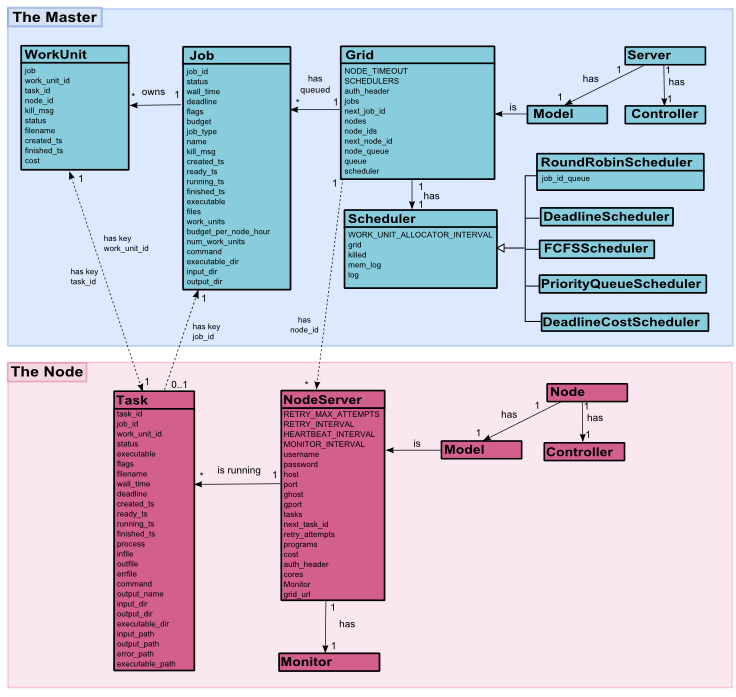
\includegraphics[keepaspectratio,width=\textwidth,height=0.75\textheight]{./figs/class.png}
\caption{New Job Creation}
\end{figure}

\section{Sequence Diagrams}

\begin{figure}[htbp]
\centering
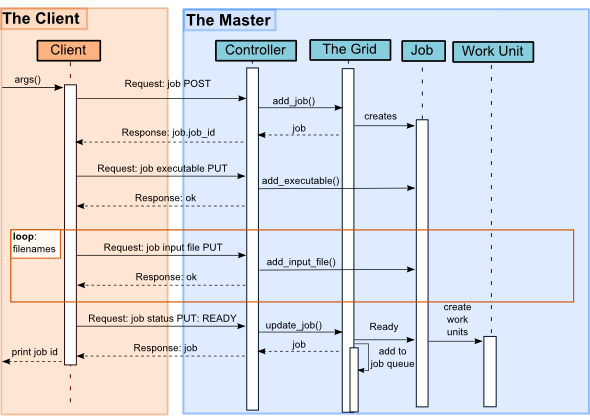
\includegraphics[keepaspectratio,width=\textwidth,height=0.75\textheight]{./figs/jobcreate.png}
\caption{New Job Creation}
\end{figure}


\begin{figure}[htbp]
\centering
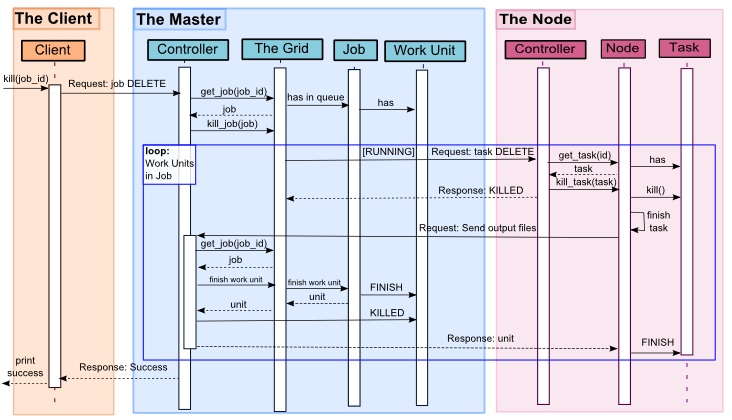
\includegraphics[keepaspectratio,width=\textwidth,height=0.75\textheight]{./figs/jobkill.png}
\caption{Kill a Job}
\end{figure}


\begin{figure}[htbp]
\centering
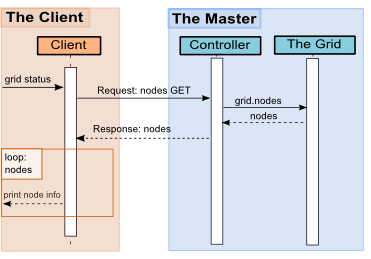
\includegraphics[keepaspectratio,width=\textwidth,height=0.75\textheight]{./figs/gridstatus.png}
\caption{Get the status of The Grid}
\end{figure}


\begin{figure}[htbp]
\centering
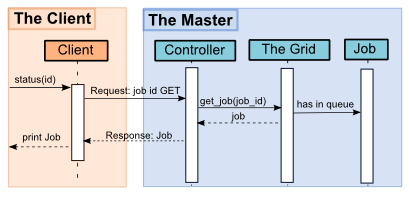
\includegraphics[keepaspectratio,width=\textwidth,height=0.75\textheight]{./figs/jobget.png}
\caption{Get the status of a Job}
\end{figure}


\begin{figure}[htbp]
\centering
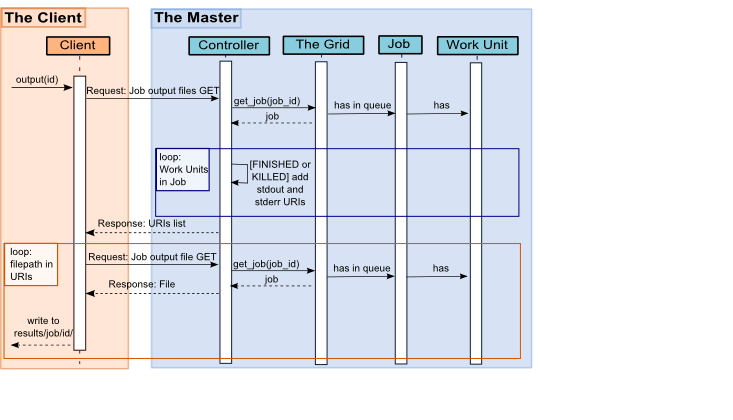
\includegraphics[keepaspectratio,width=\textwidth,height=0.75\textheight]{./figs/getoutput.png}
\caption{Get the output of a finished Job}
\end{figure}


\begin{figure}[htbp]
\centering
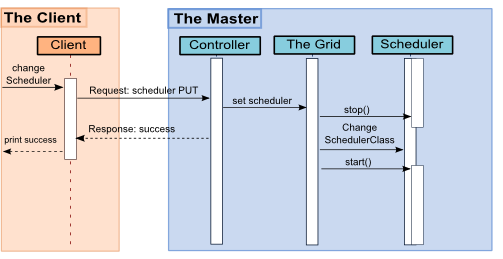
\includegraphics[keepaspectratio,width=\textwidth,height=0.75\textheight]{./figs/scheduler.png}
\caption{Change the scheduler dynamically}
\end{figure}


\begin{figure}[htbp]
\centering
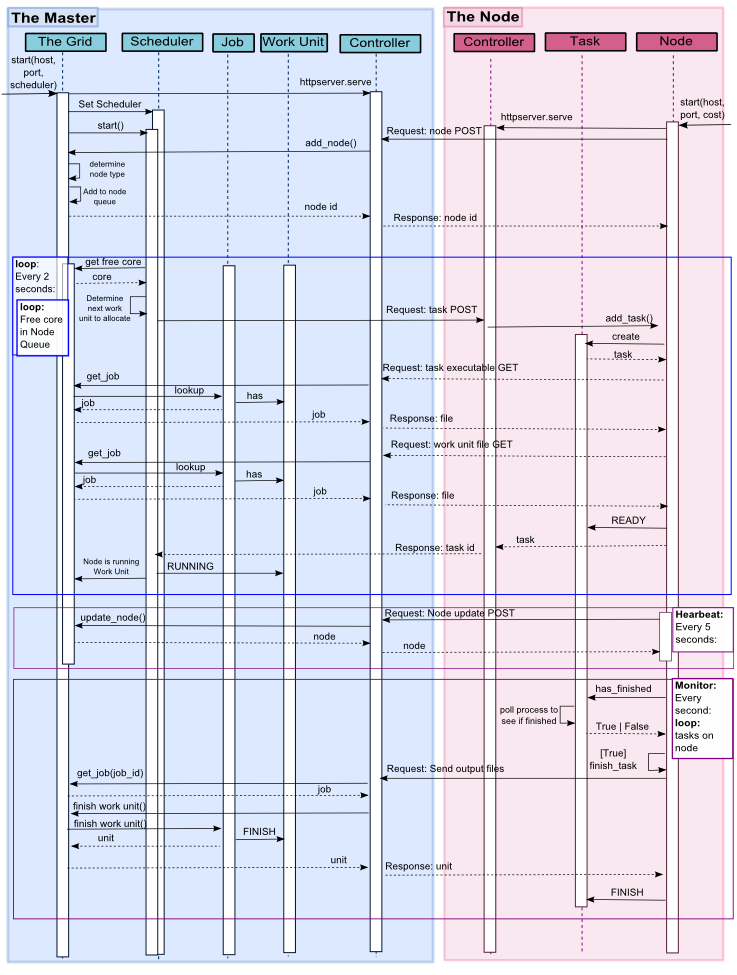
\includegraphics[keepaspectratio,width=\textwidth,height=0.75\textheight]{./figs/servernode.png}
\caption{Interaction between The Master and The Nodes in The Grid}
\end{figure}


\chapter{Implementation}
The Grid is implemented using Python 2.6, with a package dependency on Paste. Paste is a multithreaded HTTP server which is used as the underlying communication protocol in The Grid. Communication between The Client and The Master, and The Master and The Nodes is done via an agreed JSON based API. 

Python 2.6 was chosen for both internal and external reasons. Internally, the development group all knew Python better than any other language which was suitable for the task. Secondly, development in Python is quite fast, though Python itself can be quite slow. As the main latency in The Grid is in the sending of input files and executables around, the computational speed loss due to language choice was deemed negligible. Externally, Python 2.6 was chosen due to its commonly installed nature which would make it easier to install The Node software on potential nodes. 

The dependency on an external library Paste was determined nessecary, though external libraries were avoided where possible. This was done to both avoid licensing issues, as well as making the software easier to install as it needed to be portable and installed on many different environments due to the heterogenous nature of The Grid. Neither of the WSGI servers available in the standard library of Python were suitable as neither is multi-threaded, which is unworkable due to having to send possibly large files around that would otherwise block the server from accepting new requests.

The choice of HTTP to communicate over was done so because of the familiarity of the development team with HTTP based communication protocols and the development of RESTful APIs with which to communicate via JSON over HTTP. It also allowed for the easy development of a web based GUI which both had the benefit of playing to the development teams strengths as well as allowing for a interface to The Grid that is accessible anywhere in the world via the internet. HTTP also has built in authentication which was utilised in order to provided a level of security for who can access and use The Grid. HTTP is also extendible to use HTTPS which would allow for the easy securing of communication within The Grid as a possible future extension of the software.

JSON specifically was chosen as it is light-weight and easier to parse than XML, while also being easily used from within JavaScript which allowed the web service on The Master to utilise the same RESTful API as the Client and Nodes do. 

The code was developed following the MVC style architecture, though as the majority of the views are actually JSON, the majority of the code is organised into Models and Controllers. Each of the web servers on The Master and The Nodes listen to a provided list of Routes which map URIs and request type (GET, POST, PUT, DELETE) to a controller which calls any specific functions from the model and returns the relevant output JSON.

\section{The Master}
The Master instansiates a HTTP Server on a given hostname and port, which it listens on for both communications from instances of The Client as well as web requests to the Graphical User Interface provided. The Master also uses this HTTP Server to accept messages from each of The Nodes in The Grid. 

\subsection{The Scheduler}
The Master contains a Scheduler, which runs inside its own thread. It periodically polls the internal node list to see if any nodes have become available. If a node is available, it will check to see if there are any Work Units available that can be run on that node. If there is a job available, then The Scheduler will allocate the Work Unit to that node. It will then continue looking at available nodes and attempting to find available Work Units for them.

The Master contains a Scheduler, which runs inside its own thread. It periodically polls the internal node list to see if any nodes have become available. If a node is available, it will check to see if there are any Work Units available that can be run on that node. If there is a job available, then The Scheduler will allocate the Work Unit to that node. It will then continue looking at available nodes and attempting to find available Work Units for them. 

The Scheduler itself is itself contained within The Master and can be dynamically changed. In the case that a Scheduler is swapped however, the internal state unique to one Scheduler type will be lost and all jobs currently in the queue will be allocated using the new scheduling algorithm. The Scheduling algorithms available are: FCFS (First come, first served), Round Robin, Earliest Deadline First, Cost Constrained Earliest Deadline First, and Mutli-level Priority Queues. 


\subsubsection{First Come First Serve}
FCFS completes each job sequentially as they arrived. Jobs are ordered by the time they were created, and all of the Work Units in a job will be completed before Work Units from another job are executed. If a job is created but is not ready (not all files have arrived on The Master) then a job that has been created later but is ready will be executed. When the earlier job becomes ready, all Work Units from the earlier job will be executed before resuming the job that was ready first but created later. This is done as to not unfairly punish jobs with large input files by making them wait until they are ready to be considered in the queue.

\subsubsection{Round Robin}
Round Robin is similar to FCFS however rather than executing all of the Work Units from a job before moving to the next one, it iterates over the scheduled jobs, allocating them one Work Unit at a time. This is achieved by storing a persistent queue of Job IDs between polls checking the internal node list. The Work Unit from the front of this queue is allocated to a free node, and then this job ID is placed at the back of the queue. New jobs which are sent to the grid are placed at the back of the queue.

\subsubsection{Earliest Deadline First}
Earliest Deadline First takes into account the deadline of the job and prioritises jobs by earliest deadline first. That is, if a job needs to be finished by tomorrow and there is another job that can be finished in a week, then the job that needs to be finsihed by tomorrow will take preference. As Jobs are allocated by schedulers as Work Units, a job may execute some work units before a Job is created that has an earlier deadline. In this event any remaining Work Units from the already running job will be placed behind the Work Units of the new scheduler. As a jobs deadline is a fixed amount of time in the past, indefinate starvation of a job cannot occur as eventually the deadline of the job will make it the highest priority to be completed. This deadline is calculated as the job's specified deadline minus its wall time, as this is the latest date the job can start. This prevents long jobs from being starved out until they can't possibly finish by shorted jobs.

\subsubsection{Cost Constrained Earliest Deadline First}
Deadline/Cost First takes into account not only the deadline of each Work Unit as in Deadline First but also takes into account the budget of the Job. It first ensures that a job only runs on nodes that are within the Jobs budget. It secondly preferentially places jobs with higher budgets about jobs with lower budgets.

\subsubsection{Multi-level Priority Queues}
This Multi-Level Priority Queue implementation splits The Nodes on The Grid into seperate queues. There can be any number of different queues, with a different proportion of The Grid allocated to them. The default queues are Default, Batch and Fast. Half of The Nodes on The Grid are allocated to Default, which is for any generic job between 1 hour and a few days. Batch is allocated 30\% of the nodes and is for jobs that will take a week or more. Fast is allocated 20\% of the nodes and is for jobs that are less than an hour. These priorities reserve nodes for specific job types without indefinately starving any one type of job if there is an excess of another.

This scheduler also stops large jobs from taking up most of the queue during offpeak periods, and then causing a large back log of other jobs. This is an unfortunate side effect of not being able to pause and resume a Work Unit once it has begun. While Deadline First and such can interupt a low priority job in terms of stopping further execution of additional work units, if a job is already running a number of work units which each may take a long time, there is no way to interrupt these running processes.

Different scheduling algorithms are used for each of the three different types of queues. These were all cost constrained to prevent jobs from running on nodes they couldnt afford. Where two jobs were equal in the algorithm, the one with the highest budget took preference. For the Batch queue, FCFS was used because it provides high throughput. The Fast queue uses Round Robin for its good response time, and the Default queue uses Earliest Deadline First.

\section{The Node}
Each Node, like The Master, also instansiates a HTTP Server on a given hostname and port. It listens on this for communications from The Master. The Master sends job information to The Node, which in turn uses this information to request from The Master any files that The Node requires in order to complete the job it has been assigned. The Node will then execute a Work Unit once it is told by The Master that the Work Unit is READY. The Node will then preiodically check whether the Work Unit has finished executing. Once it has finished, The Node will report back to The Server that the Work Unit is complete and will then send back any information written to stdout or stderr during the Work Unit's execution.

\subsection{The Heartbeat}
The Heartbeat is a thread spawned from The Node which controls the sending of the Node's heartbeat to The Master. This heartbeat lets The Master know that The Node is still there, if this heartbeat is not received by The Master, it will be assumed to be offline. This heartbeat also detects for a loss of connection to The Master. If connection to The Master is lost, The Node will attempt to reregister itself to The Master. The Heartbeat has the additional task of monitoring the health of The Node. It reports information such as the CPU usage to The Server so that overall statistics of The Grid can be monitored at a Grid-wide level.

\subsection{The Monitor}
The Monitor is a thread spawned from The Node which monitors the state of all running processes and reports back to The Master when a Work Unit has finished executing. The Monitor will check for Jobs that may have exceeded their allotted wall time and kill them, returning their current progress.

\section{The Client}
The Client is built on top of the available API in Python and allows the creation of new Jobs via a command line interface. It additionally allows for the monitoring of a running Job's status. As well as retreiving the output files created during a Jobs execution. The Client also allows a user to kill a running job early and retrieve any output that had been generated until that point. It is also possible to dynamically modify the Scheduler being used by The Grid, however this requires the client to be logged in with an Administrator level account. The Client must be run with a provided username and password that is valid for use with The Grid. These username and password combinations can be either Client level, or Administration level. The Client level allows the user to create, view and kill jobs. The Administration level is the same as Client level, however with the additional functionality of being able to change The Scheduler.

\section{The Web Interface}
The Web Interface is built on top of the same API as The Client, however it is written with a combination of HTML and JavaScript to run from The Browser. The Web Interface is served by The Master and is accessible to any computer that can see The Master. The Web Interface has the additional feature of also being able to easily view the output log of The Scheduler, for debugging or monitoring purposes, as well as being able to see which Nodes are available, and what Work Units have been assigned to them.




\chapter{The Grid: API}
\label{thegrid:api}

Both the Web based User Interface and the Client application (Client.py) communicate with the master node of The Grid through a REST API. REST stands for Representational State Transfer and is becoming the de-facto standard for web based API's, such as those used by Twitter and Facebook. The key benefits to using this technology are that many tools exist for consuming these services; it works over HTTP enabling consumption of services on mobile devices and provides a consistent model to develop with.

Rather than using XML, we have chosen to use the JSON format. The primary driver for selecting JSON is its simplicity. XML can easily become cumbersome for development due to the challenges of maintaining XML schemas in a rapidly evolving development process. JSON is also extremely well supported within Python and Javascript which greatly simplified development.

The REST API is secured using based HTTP Authentication, preventing unauthorized access to The Grid.

\section{API End Points}
\label{apiendpoints}

\subsection{Submit Job}
\label{submitjob}

The meta-data of a job must be submitted before files can be submitted and before the job can be started.

\begin{adjustwidth}{2.5em}{2.5em}
\begin{verbatim}

URL:    /job
Method: POST
Parameters: 
    name            label for identifying the job
    wall_time       time allowance for the job (HH:MM:SS)
    deadline        date and time that the job must be completed by
    budget          amount of money this job may cost
    job_type        type of job (BATCH, FAST, DEFAULT)
Returns:    
    job_id

\end{verbatim}
\end{adjustwidth}

\subsection{Submit Executable File}
\label{submitexecutablefile}

Only a single executable file may be uploaded to the server for a particular job. If multiple files are uploaded, then latter uploads will replace the initial file.

\begin{adjustwidth}{2.5em}{2.5em}
\begin{verbatim}

URL:    /job/<job_id>/executable/<file_name>    
Method: PUT
Parameters: 
    job_id          the id of the job to submit the file to
    file_name       name of the executable file
    file_content    content of the file in the content body
Returns:    
    job_id, file_name

\end{verbatim}
\end{adjustwidth}

\subsection{Submit Input File}
\label{submitinputfile}

Many files may be associated with a single job, with the executable being executed with a single input file in each invocation which may occur on different servers.

\begin{adjustwidth}{2.5em}{2.5em}
\begin{verbatim}

URL:    /job/<job_id>/files/<file_name>
Method: PUT
Parameters: 
    job_id          the id of the job to submit the file to
    file_name       name of the executable file
    file_content    content of the file in the content body
Returns:        
    job_id, file_name

\end{verbatim}
\end{adjustwidth}

\subsection{Start Job}
\label{startjob}

After all the required files have been uploaded, the job may be started using the above mentioned url.

\begin{adjustwidth}{2.5em}{2.5em}
\begin{verbatim}

URL:    /job/<job_id>/status
Method: POST
Parameters: 
    job_id      the id of the job to start
    status      must always be "READY"
Returns:

\end{verbatim}
\end{adjustwidth}

\subsection{Kill Job}
\label{killjob}

A job may be killed when it is Queued, Ready, Pending or Running, in which case all work items that have been queued or are running will be halted. The output for jobs that have already been run will still be available.

\begin{adjustwidth}{2.5em}{2.5em}
\begin{verbatim}

URL:    /job/<job_id>
Method: DELETE
Parameters: 
    job_id      the id of the job to kill
Returns:

\end{verbatim}
\end{adjustwidth}

\subsection{List Available Nodes}
\label{listavailablenodes}

A list of all currently connected nodes is provided at this url along with the work items that each node is currently working on.

\begin{adjustwidth}{2.5em}{2.5em}
\begin{verbatim}

URL:    /node
Method: GET
Parameters:
Returns:    
    JSON encoded string listing available nodes.

\end{verbatim}
\end{adjustwidth}

\subsection{Node Information}
\label{nodeinformation}

Get all the information The Grid stores on a specific Job

\begin{adjustwidth}{2.5em}{2.5em}
\begin{verbatim}

URL:    /node/<node_id>
Method: GET
Parameters:
    node_id     the id of the node
Returns:    
    JSON encoded string of the node

\end{verbatim}
\end{adjustwidth}

\subsection{List Jobs}
\label{listjobs}

A list of all jobs that are in the pending, ready, queued, running, finished or killed state along with each jobs work items and the output files associated with those work items.

\begin{adjustwidth}{2.5em}{2.5em}
\begin{verbatim}

URL:    /job
Method: GET
Parameters:
Returns:    
    JSON encoded string listing jobs that have been submitted.

\end{verbatim}
\end{adjustwidth}

\subsection{Job Information}
\label{jobinformation}

Get all the information The Grid stores on a specific Job

\begin{adjustwidth}{2.5em}{2.5em}
\begin{verbatim}

URL:    /job/<job_id>
Method: GET
Parameters:
    job_id      the id of the job
Returns:    
    JSON encoded string of the job

\end{verbatim}
\end{adjustwidth}

\chapter{Introduction}
This report outlines the architecure, design and implementation details of The Grid, a distributed grid computing software package. The Grid allows for the distribution and exectution of self-contained executable files across a heterogenous grid, allowing users of the software to optimise the running of their jobs based on their deadline and any cost restraints. This software package includes a number of different scheduling algorithms that can be used depending on the type of jobs The Grid will be used for.

\chapter{Future Improvements}
\label{futureimprovements}

There are a number of key improvments that could make The Grid much better.

\begin{itemize}
\item The use of SSL in order to secure the communication between The Master and The Nodes and The Clients.

\item The use of a proper job specification format that would allow the sending of non-self-contained executables around the heterogenous grid.

\item The use of a virtual file system that would allow better sandboxing of executables on The Grid.

\item The allowance of more complex input\slash output execution than stdin and stdout.

\item The allowance of executables that run on more than one processor

\item The Determination of computational power at runtime to factor into Node-type load balancing. This would prevent load balancing from allocating improperly Nodes with an unusually large number of cores, RAM or processing power.

\end{itemize}

\chapter{Contributions}
\label{contributions}

Each team member of the group has contributed approximately 25\% of the work to this project. Specific leading contributions of each team member are outlined below, however all team members contributed to all aspects of the developement and design of The Grid. 

\textbf{Adam Whiteside \& Scott Richie} - Backend Communication and Framework

\textbf{Terence Siganakis} - Graphical User Interface

\textbf{Andrew Vadnal} - Scheduling Algorithms


% ============================
% Start of appendices
% ============================
\appendix

% ============================
% End of document
% ============================
\end{document}
